\begin{frame}
	\frametitle{Généralités sur XGBoost}
	\begin{center}
		XGBoost : \textit{E\textbf{X}treme \textbf{G}radient \textbf{Boost}ing}
	\end{center}
	\begin{itemize}
		\itemperso{Flexibilité}Régression, classification,...\vspace*{.2cm}
		\itemperso{Portabilité}Windows, Linux, OS X\vspace*{.2cm}
		\itemperso{Multi-langages}Python, R, JAVA, C++, Scala,...\vspace*{.2cm}
		\itemperso{Distribué}Yarn, Spark, Flink, AWS, Azure,...\vspace*{.2cm}
		\itemperso{Performance}Optimisé et expensif\vspace*{.2cm}
	\end{itemize}
\end{frame}

\begin{frame}
	\frametitle{Le boosting}
	\begin{itemize}
		\itemperso{}Une stratégie adaptative.
		\itemperso{}Convertir des règles peu performantes en (très) bonne prédiction.
		\itemperso{}Réduction variance et biais.
		\itemperso{}Convergence rapide.
		\itemperso{}Sensible au bruit.
	\end{itemize}
\end{frame}

\begin{frame}
	\frametitle{Le boosting, premier algorithme}
	\only<1>{
		\paraTitle{Premier modèle}
		\begin{center}
			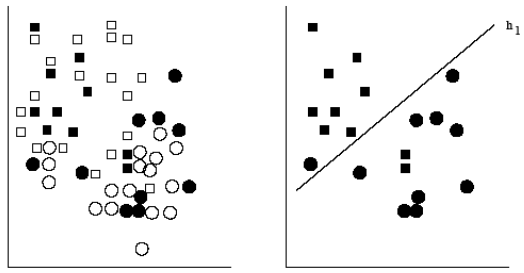
\includegraphics[height=4.5cm]{images/theorie/boosting1}
		\end{center}
		\rule{0pt}{0pt}\hfill{\fontsize{.15cm}{0cm}\selectfont\textit{Source : Cours Machine Learning, Haytham \textsc{Elghazel}}}
	}%
	\only<2>{
		\paraTitle{Deuxième modèle}
		\begin{center}
			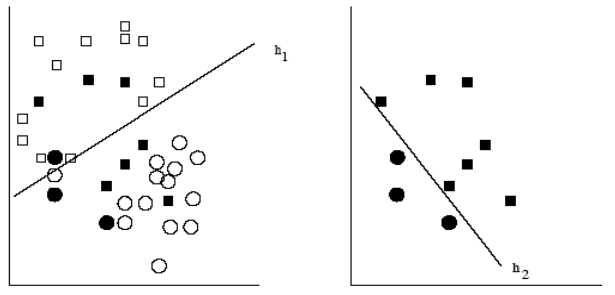
\includegraphics[height=4.5cm]{images/theorie/boosting2}
		\end{center}
		\rule{0pt}{0pt}\hfill{\fontsize{.15cm}{0cm}\selectfont\textit{Source : Cours Machine Learning, Haytham \textsc{Elghazel}}}
	}%
	\only<3>{
		\paraTitle{Troisième modèle}
		\begin{center}
			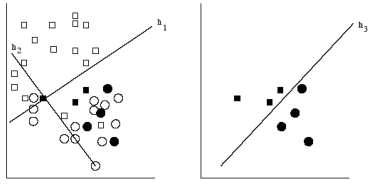
\includegraphics[height=4.5cm]{images/theorie/boosting3}
		\end{center}
		\rule{0pt}{0pt}\hfill{\fontsize{.15cm}{0cm}\selectfont\textit{Source : Cours Machine Learning, Haytham \textsc{Elghazel}}}
	}%
	\only<4>{
		\paraTitle{Vote majoritaire}
		\begin{center}
			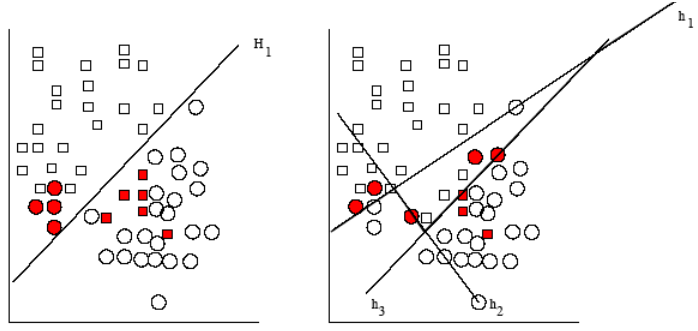
\includegraphics[height=4.5cm]{images/theorie/boosting4}
		\end{center}
		\rule{0pt}{0pt}\hfill{\fontsize{.15cm}{0cm}\selectfont\textit{Source : Cours Machine Learning, Haytham \textsc{Elghazel}}}
	}
\end{frame}

\begin{frame}
	\frametitle{Boosting et arbres}
	\only<1>{
		\paraTitle{Un arbre simple (CART)}
		\begin{center}
			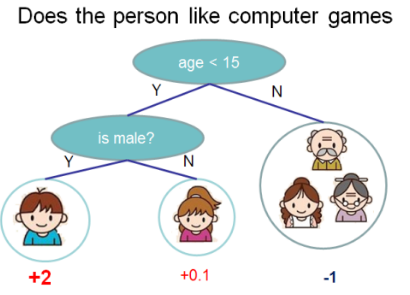
\includegraphics[height=4.5cm]{images/theorie/arbres1}
		\end{center}
		\rule{0pt}{0pt}\hfill{\fontsize{.15cm}{0cm}\selectfont\textit{Source : \texttt{https://xgboost.readthedocs.io/en/latest/model.html}}}
	}%
	\only<2>{
		\paraTitle{Plusieurs arbres vallent mieux qu'un}
		\begin{center}
			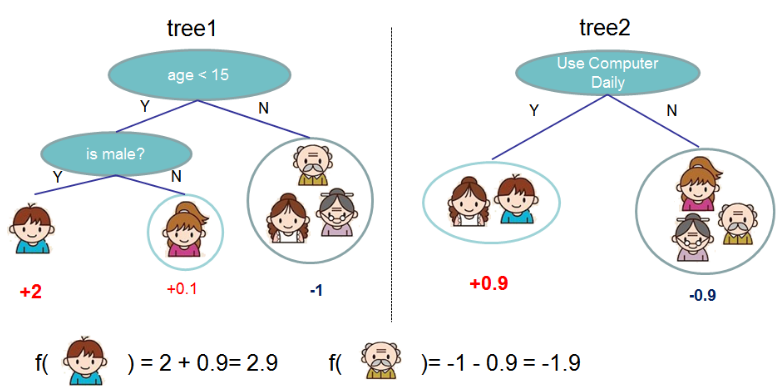
\includegraphics[height=4.5cm]{images/theorie/arbres2}
		\end{center}
		\rule{0pt}{0pt}\hfill{\fontsize{.15cm}{0cm}\selectfont\textit{Source : \texttt{https://xgboost.readthedocs.io/en/latest/model.html}}}
	}%
	\only<3-5>{
		\paraTitle{Choix de l'arbre à ajouter}
	}%
	\only<3>{
		\begin{itemize}
			\itemperso{Fonction objectif}$\textnormal{obj}(\theta)=L(\theta)+\Omega(\theta)$
		\end{itemize}
		\begin{center}
			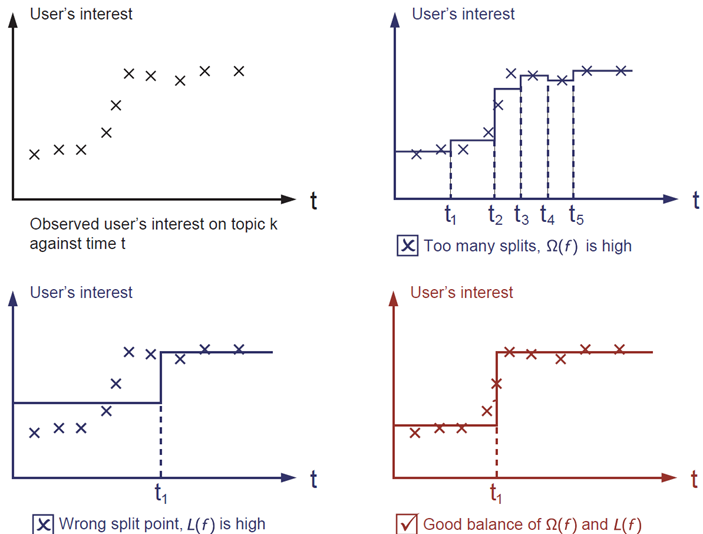
\includegraphics[width=.6\textwidth]{images/theorie/reg}
		\end{center}
		\rule{0pt}{0pt}\hfill{\fontsize{.15cm}{0cm}\selectfont\textit{Source : \texttt{https://xgboost.readthedocs.io/en/latest/model.html}}}
	}%
	\only<4>{
		\begin{itemize}
			\itemperso{Fonction de perte}$\displaystyle{L(t) = \sum_{i=1}^n\left[g_if_t(x_i)+\frac{1}{2}h_if_t^2(x_i)\right]}$
			\itemperso{Complexité}$\displaystyle{\Omega(t)=\gamma T + \frac{1}{2}\lambda\sum_{j=1}{T}\omega_j^2}$
		\end{itemize}
		\begin{center}
			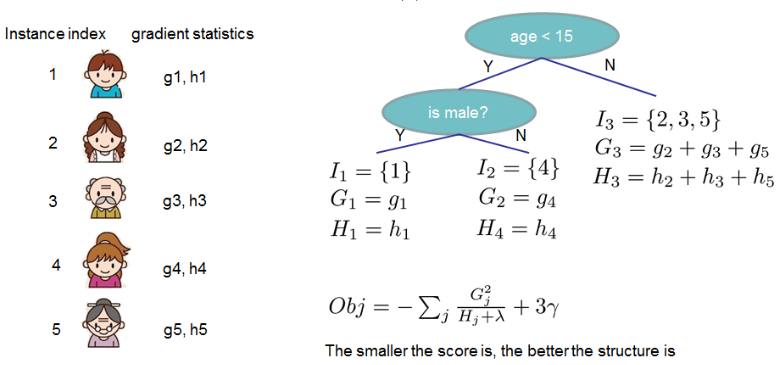
\includegraphics[width=.6\textwidth]{images/theorie/arbres3}
		\end{center}
		\rule{0pt}{0pt}\hfill{\fontsize{.15cm}{0cm}\selectfont\textit{Source : \texttt{https://xgboost.readthedocs.io/en/latest/model.html}}}
	}%
	\only<5>{
		\begin{itemize}
			\itemperso{Le gain}$\displaystyle{\frac{1}{2}\left[\frac{G_L^2}{H_L+\lambda} + \frac{G_R^2}{H_R+\lambda}-\frac{(G_L+G_R)^2}{H_L+H_R+\lambda}\right]-\gamma}$
		\end{itemize}
		\begin{center}
			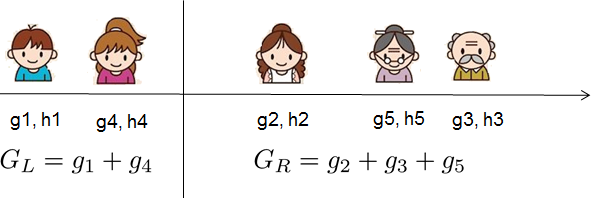
\includegraphics[width=.6\textwidth]{images/theorie/arbres4}
		\end{center}
		\rule{0pt}{0pt}\hfill{\fontsize{.15cm}{0cm}\selectfont\textit{Source : \texttt{https://xgboost.readthedocs.io/en/latest/model.html}}}
	}
\end{frame}

\begin{frame}
	\frametitle{Plus qu'une méthode de Boosting}
	\begin{itemize}
		\itemperso{}Prise en compte de la régularisation.
		\itemperso{}Calcul en parallèle.
		\itemperso{}Support de Hadoop.
		\itemperso{}Possibilité d'adaptation des fonctions objectifs.
		\itemperso{}Prise en charge des valeurs manquantes.
		\itemperso{}Version améliorée de l'élagage
		\itemperso{}Cross-validation native
	\end{itemize}
\end{frame}

\begin{frame}
	\frametitle{Performances}
	La rapidité est le but initial de XGBoost :
	\begin{itemize}
		\itemperso{Mémoire}Pas de mémoire dynamique.
		\itemperso{Cache}Utilisation respectueuse.
		\itemperso{Amélioration modèle}Voir précédemment.
		\itemperso{Conception}Parallélisation en arrière plan.
	\end{itemize}
	\rule{0pt}{0pt}\hfill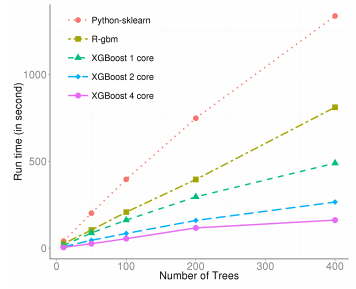
\includegraphics[width=.5\textwidth]{images/theorie/speed}\hfill\rule{0pt}{0pt}

	\rule{0pt}{0pt}\hfill{\fontsize{.15cm}{0cm}\selectfont\textit{Source : \texttt{http://www.jmlr.org/proceedings/papers/v42/chen14.pdf}}}
\end{frame}